\documentclass[12pt]{report}
\usepackage[utf8]{inputenc}
\usepackage[margin=1.2in]{geometry}
\usepackage{graphicx}
\usepackage{float}
\usepackage{subcaption}
\usepackage{amsmath}
\usepackage{amssymb}
\usepackage{ulem}
\usepackage{bm}
\usepackage{framed}
\usepackage{xcolor}
\usepackage{ragged2e}
\usepackage{color}
\usepackage{soul}
\usepackage{cancel}
\graphicspath{ {images/} }
\setlength{\parskip}{1em}
\allowdisplaybreaks


\usepackage{titling}
\newcommand{\subtitle}[1]{%
	\posttitle{%
		\par\end{center}
	\begin{center}\large#1\end{center}
	\vskip0.5em}%
}

\newenvironment{blueframed}[1][blue]
{\def\FrameCommand{\fboxsep=\FrameSep\fcolorbox{#1}{white}}%
	\MakeFramed {\advance\hsize-\width \FrameRestore}}
{\endMakeFramed}

\newenvironment{spmatrix}[1]
{\def\mysubscript{#1}\mathop\bgroup\begin{bmatrix}}
	{\end{bmatrix}\egroup_{\textstyle\mathstrut\mysubscript}}

\title{Tutorial 8}
\subtitle
{
	\textbf{keywords}: binary variables, dummy variables, intercept, slope, conditional expectation, regression line, F-test, prediction intervals, prediction uncertainty, estimation uncertainty, variation in error, sum of squared residuals, Chow test, confidence intervals, standard errors
	
	\textbf{estimated reading time}: 36 minutes
}
\author{Quang Bui}
\date{September 11, 2018}

\begin{document}
	
\maketitle

\newpage
\section*{Question 1}
\noindent \uline{Logarithmic and quadratic model}

\noindent EViews workfile: \textit{wage1tute4.wf1} from Tutorial 4

\noindent \textcolor{red}
{
	(a) Use OLS to estimate the equation
	$$log(wage) = \beta_0 + \beta_1educ + \beta_2exper + \beta_3exper^2 + u$$
	and report the results using the usual format. Name this \textbf{eq01}. [Note that in most other statistical software, you have to generate $log(wage)$ and $exper^2$ first, give them names like $lwage$ and $expersq$, then use them in the regression command. EViews allows you to do this in the regression command, which is a great advantage.]
}

\noindent To estimate this model from the \textbf{Command window} in EViews,
$$log(wage)\ c\ educ\ exper\ exper^2$$
\begin{figure}[H]
	\centering
	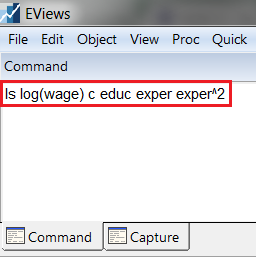
\includegraphics{tute8_q1_1}
\end{figure}
\vspace{-\baselineskip}
\noindent $$(Press\ Enter\ to\ execute\ code)$$

\noindent To name this equation \textbf{eq01},
$$Name \to Name\ to\ identify\ object: eq01$$
\begin{figure}[H]
	\centering
	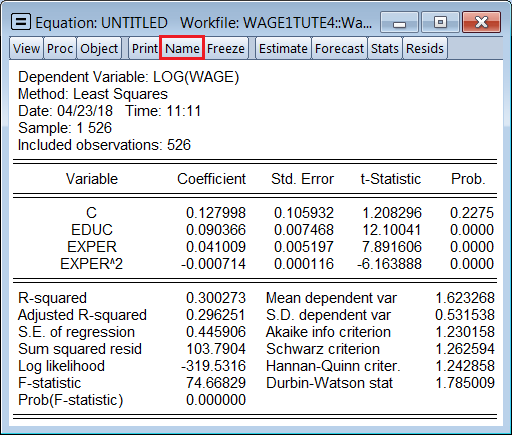
\includegraphics{tute8_q1_2}
\end{figure}
\vspace{-\baselineskip}
\begin{figure}[H]
	\centering
	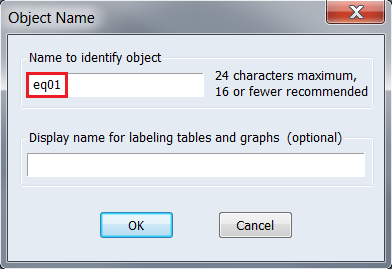
\includegraphics{q2_3}
\end{figure}
\vspace{-\baselineskip}
%%%%%%%%%% TABLE OBJECT %%%%%%%%%%
\begin{table}[H]
	\centering
	\begin{tabular}{lrrrr}
		\multicolumn{4}{l}{Dependent Variable: LOG(WAGE)}&\multicolumn{1}{c}{}\\
		\multicolumn{3}{l}{Method: Least Squares}&\multicolumn{1}{c}{}&\multicolumn{1}{c}{}\\
		\multicolumn{2}{l}{Sample: 1 526}&\multicolumn{1}{c}{}&\multicolumn{1}{c}{}&\multicolumn{1}{c}{}\\
		\multicolumn{3}{l}{Included observations: 526}&\multicolumn{1}{c}{}&\multicolumn{1}{c}{}\\
		[4.5pt] \hline \\ [-4.5pt]
		\multicolumn{1}{c}{Variable}&\multicolumn{1}{r}{Coefficient}&\multicolumn{1}{r}{Std. Error}&\multicolumn{1}{r}{t-Statistic}&\multicolumn{1}{r}{Prob.}\\
		[4.5pt] \hline \\ [-4.5pt]
		\multicolumn{1}{c}{C}&\multicolumn{1}{r}{$0.127998$}&\multicolumn{1}{r}{$0.105932$}&\multicolumn{1}{r}{$1.208296$}&\multicolumn{1}{r}{$0.2275$}\\
		\multicolumn{1}{c}{EDUC}&\multicolumn{1}{r}{$0.090366$}&\multicolumn{1}{r}{$0.007468$}&\multicolumn{1}{r}{$12.10041$}&\multicolumn{1}{r}{$0.0000$}\\
		\multicolumn{1}{c}{EXPER}&\multicolumn{1}{r}{$0.041009$}&\multicolumn{1}{r}{$0.005197$}&\multicolumn{1}{r}{$7.891606$}&\multicolumn{1}{r}{$0.0000$}\\
		\multicolumn{1}{c}{EXPER\textasciicircum 2}&\multicolumn{1}{r}{$-0.000714$}&\multicolumn{1}{r}{$0.000116$}&\multicolumn{1}{r}{$-6.163888$}&\multicolumn{1}{r}{$0.0000$}\\
		[4.5pt] \hline \\ [-4.5pt]
		\multicolumn{1}{l}{R-squared}&\multicolumn{1}{r}{$0.300273$}&\multicolumn{2}{l}{Mean dependent var}&\multicolumn{1}{r}{$1.623268$}\\
		\multicolumn{1}{l}{Adjusted R-squared}&\multicolumn{1}{r}{$0.296251$}&\multicolumn{2}{l}{S.D. dependent var}&\multicolumn{1}{r}{$0.531538$}\\
		\multicolumn{1}{l}{S.E. of regression}&\multicolumn{1}{r}{$0.445906$}&\multicolumn{2}{l}{Akaike info criterion}&\multicolumn{1}{r}{$1.230158$}\\
		\multicolumn{1}{l}{Sum squared resid}&\multicolumn{1}{r}{$103.7904$}&\multicolumn{2}{l}{Schwarz criterion}&\multicolumn{1}{r}{$1.262594$}\\
		\multicolumn{1}{l}{Log likelihood}&\multicolumn{1}{r}{$-319.5316$}&\multicolumn{2}{l}{Hannan-Quinn criter.}&\multicolumn{1}{r}{$1.242858$}\\
		\multicolumn{1}{l}{F-statistic}&\multicolumn{1}{r}{$74.66829$}&\multicolumn{2}{l}{Durbin-Watson stat}&\multicolumn{1}{r}{$1.785009$}\\
		\multicolumn{1}{l}{Prob(F-statistic)}&\multicolumn{1}{r}{$0.000000$}&\multicolumn{1}{c}{}&\multicolumn{1}{c}{}&\multicolumn{1}{c}{}\\
		[4.5pt] \hline \\ [-4.5pt]
	\end{tabular}
	%\caption{Add your caption here.}
	%\label{tab:}
\end{table}
\centering $\widehat{log(wage)} = \underset{(0.1059)}{0.1280} + \underset{(0.0075)}{0.0904}educ + \underset{(0.0052)}{0.0410}exper - \underset{(0.0001)}{0.0007}exper^2$

\justify \noindent \textcolor{red}{(b) Is $exper^2$ statistically significant at the 1\% level?}
\begin{align*}
	H_0&: \beta_3 = 0 \\
	H_1&: \beta_3 \neq 0
\end{align*}
$$t = \dfrac{\hat{\beta}_3 - \beta_{3}}{se(\hat{\beta}_3)} = \dfrac{\hat{\beta}_3 - 0}{se(\hat{\beta}_3)} = \dfrac{\hat{\beta}_3}{se(\hat{\beta}_3)} \sim t_{n-k-1} \quad under\ H_0$$
$$degrees\ of\ freedom: n-k-1 = 526-3-1 = 522$$
$$t_{calc} = \dfrac{\hat{\beta}_4}{se(\hat{\beta}_4)} = -6.1639$$
$$p-value = 0.0000$$

\newpage
\noindent Testing at the 1\% significance level,
$$\alpha = 0.01$$
$$+t_{crit} = t_{0.995,522} =$$
$$-t_{crit} = t_{0.005,522} =$$

\noindent To obtain $+t_{crit}$ in EViews,
\begin{figure}[H]
	\centering
	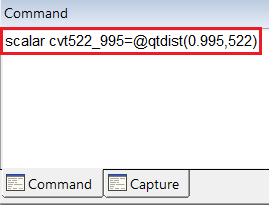
\includegraphics{q2_4}
\end{figure}
\vspace{-\baselineskip}
\begin{figure}[H]
	\centering
	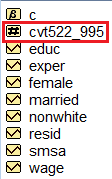
\includegraphics{q2_5}
\end{figure}
\vspace{-\baselineskip}
\begin{figure}[H]
	\centering
	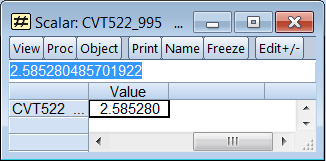
\includegraphics{q2_6}
\end{figure}
\vspace{-\baselineskip}
\noindent By comparing $t_{calc}$ with $\pm t_{crit}$, we reject $H_0$ if, $$t_{calc} > t_{crit}$$ $$OR$$ $$t_{calc} < -t_{crit}$$

\noindent Alternatively, we can compare the p-value with $\alpha$, rejecting $H_0$ if, $$p-value < \alpha$$

\noindent Since $p-value = 0.0000 < \alpha = 0.01$ we reject $H_0$ and conclude that there is sufficient evidence from our sample to suggest that $exper^2$ is statistically significant at explaining $log(wage)$ at the 1\% significance level.


\newpage
\noindent \textcolor{red}{(c) Using the approximation
	$$\%\Delta\widehat{wage} \approx 100(\hat{\beta}_2 + 2\hat{\beta}_3exper){\Delta}exper$$
	find the approximate return to the fifth year of experience. What is the approximate return to the twentieth year of experience?}

\noindent To obtain this approximation, \begin{itemize}
	\item Take the derivative of $\widehat{log(wage)}$ with respect to $exper$, $\frac{\partial\widehat{log(wage)}}{\partial exper}$
	\item Replace infinitesimally small change $\partial$ with finite change $\Delta$, $\frac{\Delta \widehat{log(wage)}}{\Delta exper}$
	\item Multiple 100 on both sides
	\item Multiple $\Delta exper$ on both sides
\end{itemize}

\noindent Return to $5^{th}$ year of experience:
\begin{align*}	
exper &= 4 \\
{\Delta}exper &= 1 \\
\%\Delta\widehat{wage} &\approx 100(\hat{\beta}_2 + 2\hat{\beta}_3 \times 4)\times 1 \\
&= 3.5\%
\end{align*}
\noindent Return to $20^{th}$ year of experience:
\begin{align*}	
exper &= 19 \\
{\Delta}exper &= 1 \\
\%\Delta\widehat{wage} &\approx 100(\hat{\beta}_2 + 2\hat{\beta}_3 \times 19)\times 1 \\
&= 1.4\%
\end{align*}
\noindent We can see that that percentage return on wage for each additional year of experience diminishes.

\noindent \textcolor{red}{(d) At what value of $exper$ does additional experience actually lower predicted $log(wage)$? How many people have more experience in this sample?}
$$\widehat{log(wage)} = \hat{\beta}_0 + \hat{\beta}_1educ + \hat{\beta}_2exper + \hat{\beta}_3exper^2 $$
$$\dfrac{\partial\widehat{log(wage)}}{{\partial}exper} = \hat{\beta}_2 + 2\hat{\beta}_3exper \qquad Let,\ \dfrac{\partial\widehat{log(wage)}}{{\partial}exper} = 0\ solve\ for\ exper$$
$$\hat{\beta}_2 + 2\hat{\beta}_3exper = 0 $$
$$exper =  -\dfrac{\hat{\beta}_2}{2\hat{\beta}_3} = \dfrac{0.0410}{2\times0.0007} \approx 29\ years\ of\ experience$$

\newpage
\section*{Question 2}
\noindent EViews workfile: \textit{marks.wf1}

\noindent The data set \textit{marks.wf1} contains data on students’ performance in a previous year in Introductory Econometrics. The variables are:
\begin{align*}
	exam &- final\ mark\ in\ exam\ (\%) \\
	asgnmt &- mark\ on\ assignments\ (\%) \\
	etc3440 &- 1\ for\ students\ in\ ETC3440, 0\ for\ students\ in\ ETC2410
\end{align*}
\noindent There were no students taking Introductory Econometrics under any other code in that year. The goal is to make a predictive model that uses assignment mark to predict final exam mark.

\noindent \textcolor{red}{(a) ``Look at the data." Do you see any anomalies in the final exam marks? If so, discuss what you would do about it.}

\noindent To visualise the distribution of final exam marks (histogram) and obtain some descriptive statistics,
$$Double\ click\ on\ exam$$
\begin{figure}[H]
	\centering
	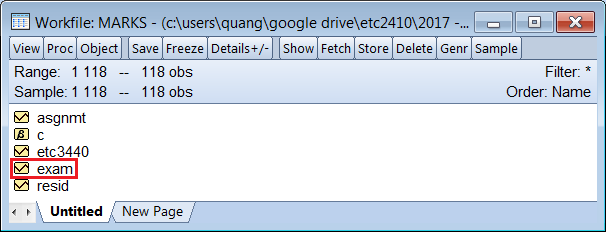
\includegraphics{q1_1}
\end{figure}
\vspace{-\baselineskip}
$$View\ \to Descriptive\ Statistics\ \&\ Tests\ \to Histograms\ and\ Stats$$
\begin{figure}[H]
	\centerline{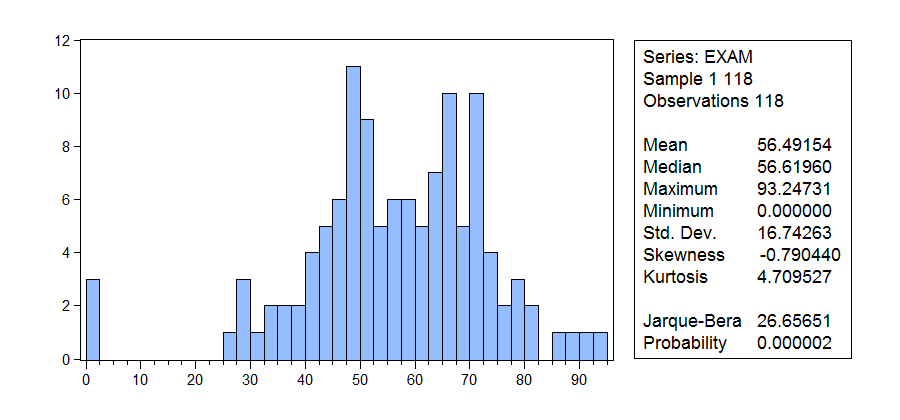
\includegraphics{q1_2}}
	\caption{Histogram and descriptive statistics of final exam mark (\%).}
\end{figure}
\vspace{-\baselineskip}

\noindent We observe 3 students with an exam mark of 0. These may have been students with very special consideration or ones that did not attend the exam, so we will omit these observations as they will affect the estimate of correlation between assignment mark and final exam mark, and $\therefore$ our estimated predictive model.

\noindent To omit these observations from our EViews sample,
$$Workfile \to Sample$$
\begin{figure}[H]
	\centering
	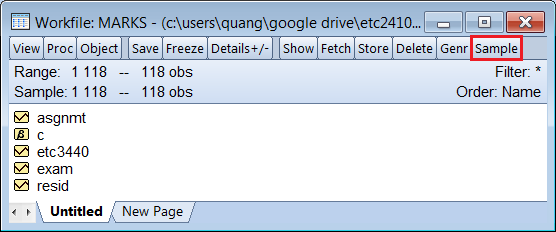
\includegraphics{q1_3}
\end{figure}
\vspace{-\baselineskip}
$$IF\ condition\ (optional): exam>0$$
\begin{figure}[H]
	\centering
	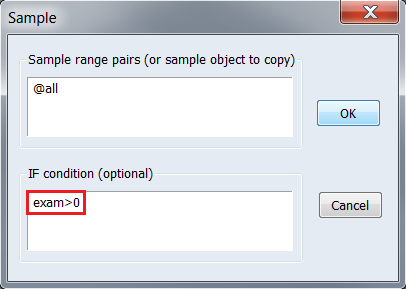
\includegraphics{q1_4}
\end{figure}
\vspace{-\baselineskip}
\noindent The workfile sample now contains only students who scored higher than 0 in their final exam.
\begin{figure}[H]
	\centering
	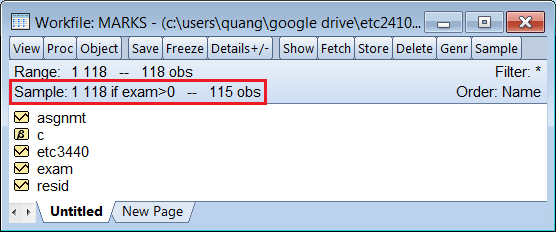
\includegraphics{q1_5}
\end{figure}
\vspace{-\baselineskip}

\newpage
\noindent \textcolor{red}
{
	(b) By using the dummy variable $etc3440$ in a regression, test if there is any difference between the expected exam mark in ETC2410 and ETC3440.
}
\justify
\begin{blueframed}
	\textcolor{blue}{\textbf{Background}}
	\vspace{-\baselineskip}
	\justify
	\textcolor{blue}{\underline{Conditional expectation with dummy variables}}
	
	\noindent \textcolor{blue}{For the simple regression model,$$exam = \beta_0 + \beta_1etc3440 + u$$ the expectation of exam score conditional on whether the student is enrolled in ETC2410 or ETC3440 is given by,
		$$E(exam|etc3440) = \beta_0 + \beta_1etc3440$$
		$\therefore$ the expected exam score if the student is enrolled in ETC3440, $$E(exam|etc3440=1) = \beta_0 + \beta_1{\times}1 = \beta_0 + \beta_1$$
		and the expected exam score if the student is enrolled in ETC2410, $$E(exam|etc3440=0) = \beta_0 + \beta_1{\times}0 = \beta_0$$ If there is no difference between the expected exam score for ETC3440 and ETC2410 students then, $$E(exam|etc3440=1) = E(exam|etc3440=0)$$ i.e.,
		$$\beta_1 = 0$$
		otherwise,
		$$\beta_1 \neq 0$$
	}
\end{blueframed}
\centering $exam = \beta_0 + \beta_1etc3440 + u$
\justify \noindent To estimate this model from the \textbf{Command window},
$$ls\ exam\ c\ etc3440$$
\begin{figure}[H]
	\centering
	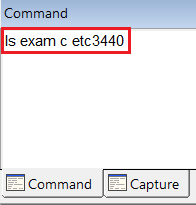
\includegraphics{q1_6}
\end{figure}
\vspace{-\baselineskip}
$$(Press\ Enter\ to\ execute\ code)$$
\begin{figure}[H]
	\centering
	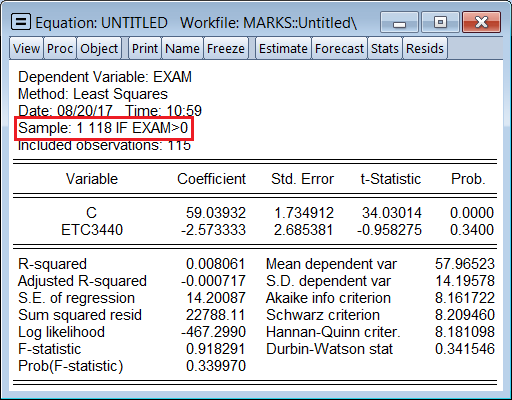
\includegraphics{q1_7}
\end{figure}
\vspace{-\baselineskip}
\noindent To name (save) the estimated equation,
$$Name \to Name\ to\ identify\ object: eq01$$
$$(This\ names\ the\ equation\ \textit{\textbf{eq01}})$$
\begin{figure}[H]
	\centering
	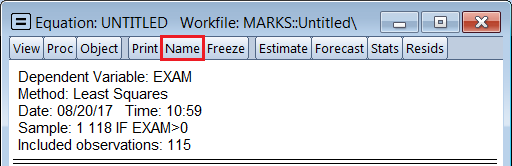
\includegraphics{q1_8}
\end{figure}
\vspace{-\baselineskip}
\begin{figure}[H]
	\centering
	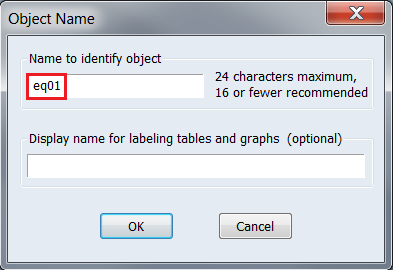
\includegraphics{q1_9}
\end{figure}
\vspace{-\baselineskip}
%%%%%%%%%% TABLE OBJECT %%%%%%%%%%
\begin{table}[H]
	\centering
	\begin{tabular}{lrrrr}
		\multicolumn{3}{l}{Dependent Variable: EXAM}&\multicolumn{1}{c}{}&\multicolumn{1}{c}{}\\
		\multicolumn{3}{l}{Method: Least Squares}&\multicolumn{1}{c}{}&\multicolumn{1}{c}{}\\
		\multicolumn{3}{l}{Sample: 1 118 IF EXAM\textgreater 0}&\multicolumn{1}{c}{}&\multicolumn{1}{c}{}\\
		\multicolumn{3}{l}{Included observations: 115}&\multicolumn{1}{c}{}&\multicolumn{1}{c}{}\\
		[4.5pt] \hline \\ [-4.5pt]
		\multicolumn{1}{c}{Variable}&\multicolumn{1}{r}{Coefficient}&\multicolumn{1}{r}{Std. Error}&\multicolumn{1}{r}{t-Statistic}&\multicolumn{1}{r}{Prob.}\\
		[4.5pt] \hline \\ [-4.5pt]
		\multicolumn{1}{c}{C}&\multicolumn{1}{r}{$59.03932$}&\multicolumn{1}{r}{$1.734912$}&\multicolumn{1}{r}{$34.03014$}&\multicolumn{1}{r}{$0.0000$}\\
		\multicolumn{1}{c}{ETC3440}&\multicolumn{1}{r}{$-2.573333$}&\multicolumn{1}{r}{$2.685381$}&\multicolumn{1}{r}{$-0.958275$}&\multicolumn{1}{r}{$0.3400$}\\
		[4.5pt] \hline \\ [-4.5pt]
		\multicolumn{1}{l}{R-squared}&\multicolumn{1}{r}{$0.008061$}&\multicolumn{2}{l}{Mean dependent var}&\multicolumn{1}{r}{$57.96523$}\\
		\multicolumn{1}{l}{Adjusted R-squared}&\multicolumn{1}{r}{$-0.000717$}&\multicolumn{2}{l}{S.D. dependent var}&\multicolumn{1}{r}{$14.19578$}\\
		\multicolumn{1}{l}{S.E. of regression}&\multicolumn{1}{r}{$14.20087$}&\multicolumn{2}{l}{Akaike info criterion}&\multicolumn{1}{r}{$8.161722$}\\
		\multicolumn{1}{l}{Sum squared resid}&\multicolumn{1}{r}{$22788.11$}&\multicolumn{2}{l}{Schwarz criterion}&\multicolumn{1}{r}{$8.209460$}\\
		\multicolumn{1}{l}{Log likelihood}&\multicolumn{1}{r}{$-467.2990$}&\multicolumn{2}{l}{Hannan-Quinn criter.}&\multicolumn{1}{r}{$8.181098$}\\
		\multicolumn{1}{l}{F-statistic}&\multicolumn{1}{r}{$0.918291$}&\multicolumn{2}{l}{Durbin-Watson stat}&\multicolumn{1}{r}{$0.341546$}\\
		\multicolumn{1}{l}{Prob(F-statistic)}&\multicolumn{1}{r}{$0.339970$}&\multicolumn{1}{c}{}&\multicolumn{1}{c}{}&\multicolumn{1}{c}{}\\
		[4.5pt] \hline \\ [-4.5pt]
	\end{tabular}
	%\caption{Regression output of $exam$ on constant and $etc3440$.}
	%\label{tab:}
\end{table}
\vspace{-\baselineskip} \centering$\widehat{exam} = \underset{(1.7349)}{59.0393} - \underset{(2.6854)}{2.5733}etc3440$

\justify \noindent \textbf{State the null and alternative hypothesis}
\begin{align*}
H_0&: \beta_1 = 0 \quad (no\ difference\ in\ exam\ mark\ between\ ETC3440\ and\ ETC2410\ students) \\
H_1&: \beta_1 \neq 0 \quad (difference\ in\ exam\ mark\ between\ ETC3440\ and\ ETC2410\ students)
\end{align*}
\noindent \textbf{The test statistic and its distribution under $H_0$}
$$t = \dfrac{\hat{\beta}_1 - \beta_1}{se(\hat{\beta}_1)} = \dfrac{\hat{\beta}_1}{se(\hat{\beta}_1)} \sim t_{n-k-1} \quad under\ H_0$$
\begin{align*}
n &= sample\ size = 115 \\
k &= number\ of\ regressors = 2
\end{align*}

\noindent \textbf{Calculate the test statistic}
$$t_{calc} = -\dfrac{2.5733}{2.6854} = -0.9583$$
\begin{figure}[H]
	\centering
	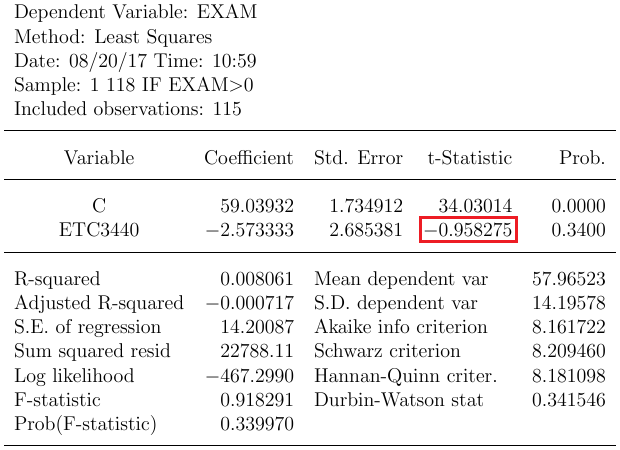
\includegraphics{q1_10}
\end{figure}
\vspace{-\baselineskip}
\noindent \textbf{p-value}
$$p-value = 0.3400$$

\noindent Note: The $Prob.$ values from the EViews regression output are p-values for a two-sided t-test to test if a regressor is statistically significant, holding the other regressors constant.

\noindent \textbf{Critical value and rejection region}

\noindent To obtain the critical value using the Stats Table, locate the t distribution table,
$$degrees\ of\ freedom = 113$$
\noindent Since 169 is not in the table, we take a conservative approach and choose the closest available degrees of freedom less than 113 i.e. $d.o.f=90$. 
\begin{figure}[H]
	\centering
	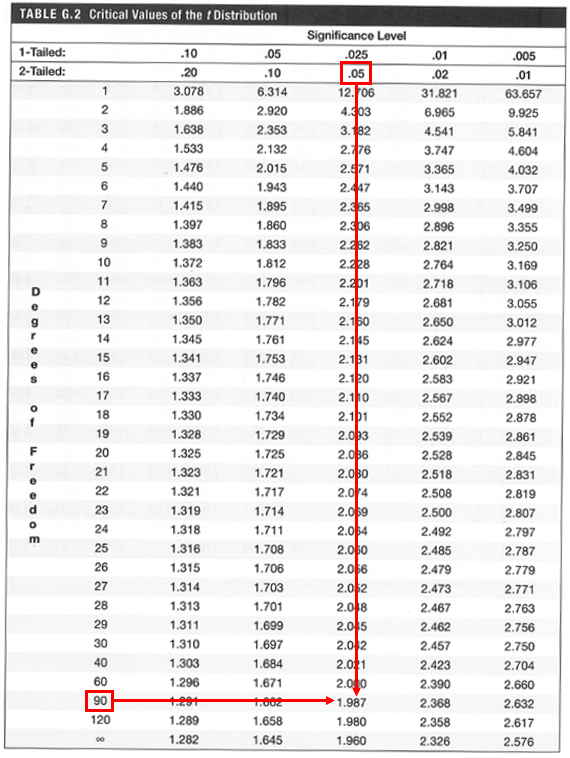
\includegraphics{q1_11}
\end{figure}
\vspace{-\baselineskip}
\noindent To obtain the critical value using EViews,
$$Command\ window:\ scalar\ cvt113\_5\_twotail=@qtdist(0.975,113)$$
\begin{figure}[H]
	\centering
	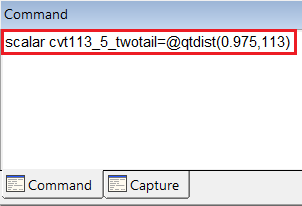
\includegraphics{q1_12}
\end{figure}
\vspace{-\baselineskip}
\begin{figure}[H]
	\centering
	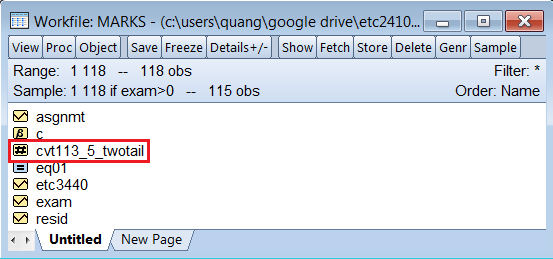
\includegraphics{q1_13}
\end{figure}
\vspace{-\baselineskip}
\begin{figure}[H]
	\centering
	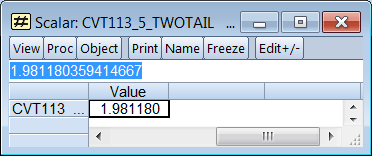
\includegraphics{q1_14}
\end{figure}
\vspace{-\baselineskip}
\noindent From Stat Table:
\begin{align*}
+t_{crit} &= 1.987 \\
-t_{crit} &= -1.987
\end{align*}
\noindent From EViews:
\begin{align*}
+t_{crit} &= 1.9812 \\
-t_{crit} &= -1.9812
\end{align*}

\noindent Rejection rule: 

\noindent Comparing the calculated test statistic with the critical value, we reject $H_0$ if,
$$t_{calc} > +t_{crit}$$
$$or$$
$$t_{calc} < -t_{crit}$$

\noindent Comparing the p-value with the significance level, we reject $H_0$ if,
$$p-value < \alpha = 0.05$$

\noindent \textbf{Conclusion}

\noindent Since $p-value = 0.3400 > \alpha = 0.05$, we do not reject the null at the 5\% significance level and conclude that there is insufficient evidence from our sample to suggest that there is a difference in expected exam mark between ETC3440 and ETC2410 students.

\newpage
\noindent \textcolor{red}
{
	(c) Estimate a regression of $exam$ on a constant and $asgnmt$,$$exam = \beta_0 + \beta_1asgnmt + u$$ along with the scatter plot with regression line added. \\ \\ Based on this regression, provide predictions for the exam marks of a student who has obtained 40\% on the assignment, and another student who has obtained 80\% on the assignment. \\ \\ Provide 95\% prediction intervals for the exam mark, once ignoring estimation uncertainty, and once properly accounting for estimation uncertainty.
}

\noindent To estimate this model from the Command window,
$$ls\ exam\ c\ asgnmt$$
\begin{figure}[H]
	\centering
	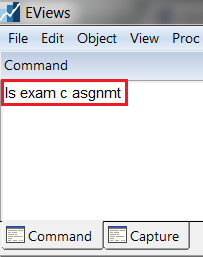
\includegraphics{tute8_q2_1}
\end{figure}
\vspace{-\baselineskip}
$$(Press\ Enter\ to\ execute\ code)$$
\noindent To name (save) the estimated equation,
$$Name \to Name\ to\ identify\ object: eq02$$
$$(This\ names\ the\ equation\ \textit{\textbf{eq02}})$$
\begin{figure}[H]
	\centering
	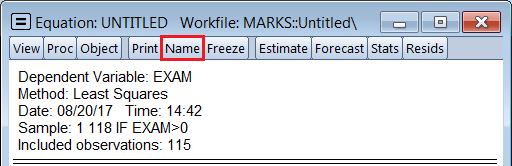
\includegraphics{q1_16}
\end{figure}
\vspace{-\baselineskip}
\begin{figure}[H]
	\centering
	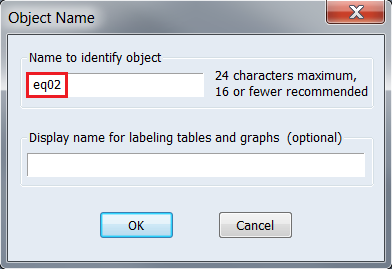
\includegraphics{q1_17}
\end{figure}
\vspace{-\baselineskip}
%%%%%%%%%% TABLE OBJECT %%%%%%%%%%
\begin{table}[H]
	\centering
	\begin{tabular}{lrrrr}
		\multicolumn{3}{l}{Dependent Variable: EXAM}&\multicolumn{1}{c}{}&\multicolumn{1}{c}{}\\
		\multicolumn{3}{l}{Method: Least Squares}&\multicolumn{1}{c}{}&\multicolumn{1}{c}{}\\
		\multicolumn{3}{l}{Date: 04/23/18   Time: 13:40}&\multicolumn{1}{c}{}&\multicolumn{1}{c}{}\\
		\multicolumn{3}{l}{Sample: 1 118 IF EXAM\textgreater 0}&\multicolumn{1}{c}{}&\multicolumn{1}{c}{}\\
		\multicolumn{3}{l}{Included observations: 115}&\multicolumn{1}{c}{}&\multicolumn{1}{c}{}\\
		[4.5pt] \hline \\ [-4.5pt]
		\multicolumn{1}{c}{Variable}&\multicolumn{1}{r}{Coefficient}&\multicolumn{1}{r}{Std. Error}&\multicolumn{1}{r}{t-Statistic}&\multicolumn{1}{r}{Prob.}\\
		[4.5pt] \hline \\ [-4.5pt]
		\multicolumn{1}{c}{C}&\multicolumn{1}{r}{$20.04634$}&\multicolumn{1}{r}{$4.876848$}&\multicolumn{1}{r}{$4.110512$}&\multicolumn{1}{r}{$0.0001$}\\
		\multicolumn{1}{c}{ASGNMT}&\multicolumn{1}{r}{$0.638077$}&\multicolumn{1}{r}{$0.080088$}&\multicolumn{1}{r}{$7.967197$}&\multicolumn{1}{r}{$0.0000$}\\
		[4.5pt] \hline \\ [-4.5pt]
		\multicolumn{1}{l}{R-squared}&\multicolumn{1}{r}{$0.359687$}&\multicolumn{2}{l}{Mean dependent var}&\multicolumn{1}{r}{$57.96523$}\\
		\multicolumn{1}{l}{Adjusted R-squared}&\multicolumn{1}{r}{$0.354021$}&\multicolumn{2}{l}{S.D. dependent var}&\multicolumn{1}{r}{$14.19578$}\\
		\multicolumn{1}{l}{S.E. of regression}&\multicolumn{1}{r}{$11.40955$}&\multicolumn{2}{l}{Akaike info criterion}&\multicolumn{1}{r}{$7.724017$}\\
		\multicolumn{1}{l}{Sum squared resid}&\multicolumn{1}{r}{$14710.10$}&\multicolumn{2}{l}{Schwarz criterion}&\multicolumn{1}{r}{$7.771755$}\\
		\multicolumn{1}{l}{Log likelihood}&\multicolumn{1}{r}{$-442.1310$}&\multicolumn{2}{l}{Hannan-Quinn criter.}&\multicolumn{1}{r}{$7.743394$}\\
		\multicolumn{1}{l}{F-statistic}&\multicolumn{1}{r}{$63.47622$}&\multicolumn{2}{l}{Durbin-Watson stat}&\multicolumn{1}{r}{$1.240656$}\\
		\multicolumn{1}{l}{Prob(F-statistic)}&\multicolumn{1}{r}{$0.000000$}&\multicolumn{1}{c}{}&\multicolumn{1}{c}{}&\multicolumn{1}{c}{}\\
		[4.5pt] \hline \\ [-4.5pt]
	\end{tabular}
	%\caption{Add your caption here.}
	%\label{tab:}
\end{table}

\vspace{-\baselineskip}
\centering $\widehat{exam} = \underset{(4.8768)}{20.0463} + \underset{(0.0801)}{0.6381}asgnmt$
\justify \noindent To obtain a scatter plot of $exam$ against $asgnmt$ with a regression line,
$$Quick \to Graph...$$
\begin{figure}[H]
	\centering
	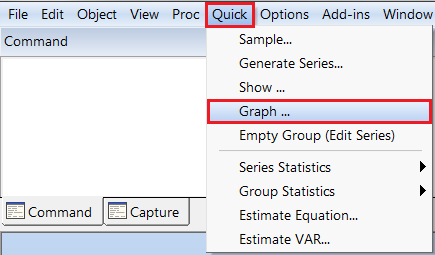
\includegraphics{q1_18}
\end{figure}
\vspace{-\baselineskip}
$$Series\ List:\ asgnmt\ exam$$
\begin{figure}[H]
	\centering
	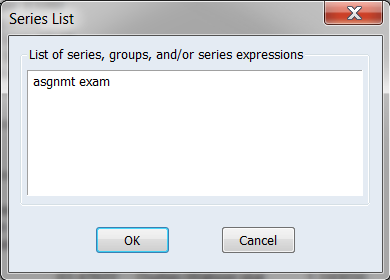
\includegraphics{q1_19}
\end{figure}
\vspace{-\baselineskip}
$$Specific:\ Scatter\ \to Fit\ lines:\ Regression\ Line$$
\begin{figure}[H]
	\centering
	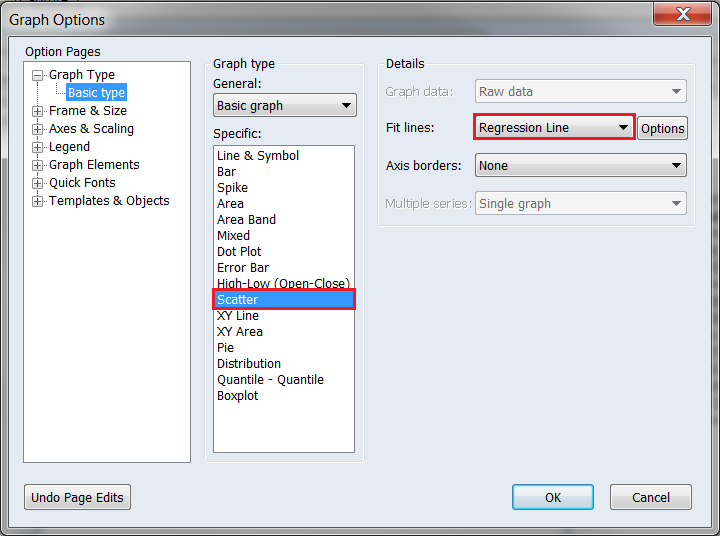
\includegraphics{q1_20}
\end{figure}
\vspace{-\baselineskip}
\begin{figure}[H]
	\centering
	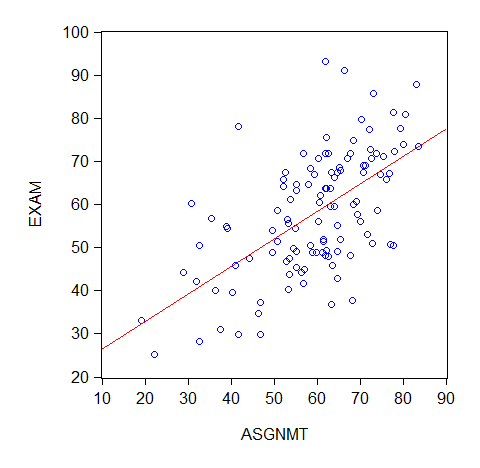
\includegraphics{q1_21}
	\caption{Scatter plot of final exam mark against assignment mark.}
\end{figure}
\vspace{-\baselineskip}
\noindent \textcolor{red}
{
	Based on this regression, provide predictions for the exam marks of a student who has obtained 40\% on the assignment, and another student who has obtained 80\% on the assignment.
}
$$exam = \beta_0 + \beta_1 asgnmt + u$$ $$E(exam|asgnmt) = \beta_0 + \beta_1 asgnmts$$
\begin{align*}
	\widehat{exam} &= \widehat{E(exam|asgnmt}) \\
	&= \hat{\beta}_0 + \hat{\beta}_1 asgnmt
\end{align*}
\noindent $\widehat{exam}$ plays two roles: 
\begin{itemize}
	\item It is the prediction of final exam score given an assignment score
	\item And also the estimated expectation of final exam score conditional on assignment score
\end{itemize}

\noindent Prediction of exam mark for a student that scored 40\% on the assignment:
\begin{align*}
	\widehat{exam} &= \widehat{E(exam|asgnmt = 40)} \\
	&= 20.0463 + 0.6381{\times}40 \\
	&= 45.5703
\end{align*}

\noindent Prediction of exam mark for a student that scored 80\% on the assignment:
\begin{align*}
\widehat{exam} &= \widehat{E(exam|asgnmt = 80)} \\
&= 20.0463 + 0.6381{\times}80 \\
&= 71.0925
\end{align*}

\noindent By regressing $exam$ on a constant and $(asgnmt-80)$,
$$exam = \beta_0 + \beta_1(asgnmt-80) + u$$
\begin{figure}[H]
	\centering
	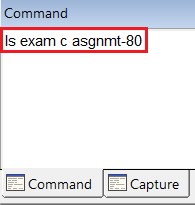
\includegraphics{q1_22}
\end{figure}
\vspace{-\baselineskip}
%%%%%%%%%% TABLE OBJECT %%%%%%%%%%
\begin{table}[H]
	\centering
	\begin{tabular}{lrrrr}
		\multicolumn{3}{l}{Dependent Variable: EXAM}&\multicolumn{1}{c}{}&\multicolumn{1}{c}{}\\
		\multicolumn{3}{l}{Method: Least Squares}&\multicolumn{1}{c}{}&\multicolumn{1}{c}{}\\
		\multicolumn{3}{l}{Sample: 1 118 IF EXAM\textgreater 0}&\multicolumn{1}{c}{}&\multicolumn{1}{c}{}\\
		\multicolumn{3}{l}{Included observations: 115}&\multicolumn{1}{c}{}&\multicolumn{1}{c}{}\\
		[4.5pt] \hline \\ [-4.5pt]
		\multicolumn{1}{c}{Variable}&\multicolumn{1}{r}{Coefficient}&\multicolumn{1}{r}{Std. Error}&\multicolumn{1}{r}{t-Statistic}&\multicolumn{1}{r}{Prob.}\\
		[4.5pt] \hline \\ [-4.5pt]
		\multicolumn{1}{c}{C}&\multicolumn{1}{r}{$71.09253$}&\multicolumn{1}{r}{$1.961324$}&\multicolumn{1}{r}{$36.24721$}&\multicolumn{1}{r}{$0.0000$}\\
		\multicolumn{1}{c}{ASGNMT-80}&\multicolumn{1}{r}{$0.638077$}&\multicolumn{1}{r}{$0.080088$}&\multicolumn{1}{r}{$7.967197$}&\multicolumn{1}{r}{$0.0000$}\\
		[4.5pt] \hline \\ [-4.5pt]
		\multicolumn{1}{l}{R-squared}&\multicolumn{1}{r}{$0.359687$}&\multicolumn{2}{l}{Mean dependent var}&\multicolumn{1}{r}{$57.96523$}\\
		\multicolumn{1}{l}{Adjusted R-squared}&\multicolumn{1}{r}{$0.354021$}&\multicolumn{2}{l}{S.D. dependent var}&\multicolumn{1}{r}{$14.19578$}\\
		\multicolumn{1}{l}{S.E. of regression}&\multicolumn{1}{r}{$11.40955$}&\multicolumn{2}{l}{Akaike info criterion}&\multicolumn{1}{r}{$7.724017$}\\
		\multicolumn{1}{l}{Sum squared resid}&\multicolumn{1}{r}{$14710.10$}&\multicolumn{2}{l}{Schwarz criterion}&\multicolumn{1}{r}{$7.771755$}\\
		\multicolumn{1}{l}{Log likelihood}&\multicolumn{1}{r}{$-442.1310$}&\multicolumn{2}{l}{Hannan-Quinn criter.}&\multicolumn{1}{r}{$7.743394$}\\
		\multicolumn{1}{l}{F-statistic}&\multicolumn{1}{r}{$63.47622$}&\multicolumn{2}{l}{Durbin-Watson stat}&\multicolumn{1}{r}{$1.240656$}\\
		\multicolumn{1}{l}{Prob(F-statistic)}&\multicolumn{1}{r}{$0.000000$}&\multicolumn{1}{c}{}&\multicolumn{1}{c}{}&\multicolumn{1}{c}{}\\
		[4.5pt] \hline \\ [-4.5pt]
	\end{tabular}
	%\caption{Regression output of $exam$ on a constant and $asgnmt-80$.}
	%\label{tab:}
\end{table}
\vspace{-\baselineskip}
\centering $\widehat{exam} = \underset{(1.9613)}{71.0925} + \underset{(0.0801)}{0.6381}(asgnmt-80)$

\justify \noindent $\hat{\beta}_0$ becomes the prediction of final exam mark for a student that scored 80\% on the assignment, and $se(\hat{\beta}_0)$ becomes the standard error of the prediction of final exam mark for a student scored 80\% on the assignment.

\noindent \textcolor{red}
{
	Provide 95\% prediction intervals for the exam mark, once ignoring estimation uncertainty, and once properly accounting for estimation uncertainty.
}

\justify
\begin{blueframed}
	\textcolor{blue}{\textbf{Background}}
	\vspace{-\baselineskip}
	\justify
	\textcolor{blue}{\underline{Prediction Uncertainty}}
	
	\noindent \textcolor{blue}
	{
		For the following simple regression model, $$exam = \beta_0 + \beta_1asgnmt + u$$
		The expectation of $exam$ conditional on $asgnmt$ is given by,
		\begin{align*}
		E(exam|asgnmt) &= E(\beta_0 + \beta_1asgnmt + u|asgnmt) \\
		&= \beta_0 + \beta_1asgnmt + E(u|asgnmt) \\ 
		&= \beta_0 + \beta_1asgnmt
		\end{align*}
		The true final exam mark given that \textit{assignment score is 80},
		$$exam = \beta_0 + 80\beta_1 + u$$
		Let $\widehat{exam}$ be the prediction of final exam mark for an \textit{assignment score of 80},
		\begin{align*}
		\widehat{exam} &= \hat{\beta}_0 + 80\hat{\beta}_1 
		\end{align*}
		which is also equal to the estimated expectation of exam mark given an \textit{assignment score of 80},
		$$\widehat{E(exam|asgnmt=80)} = \hat{\beta}_0 + 80\hat{\beta}_1$$
		Since $\widehat{exam} = \widehat{E(exam|asgnmt=80)}$ depends on $\hat{\beta}_0$ and $\hat{\beta}_1$, the OLS estimator for $\beta_0$ and $\beta_1$,
		$$\boldsymbol{\hat{\beta}} = (\textit{\textbf{X}}'\textit{\textbf{X}})^{-1}\textit{\textbf{X}}'\textit{\textbf{y}} 
		= 
		\begin{bmatrix}
		\hat{\beta}_0 \\
		\hat{\beta}_1 
		\end{bmatrix} $$
		is subject to sampling variation (since it is a random variable and varies from sample to sample), so it follows that, $$\widehat{exam} = \hat{\beta}_0 + 80\hat{\beta}_1$$ (the prediction of final exam mark for a student with an assignment score of 80) is also subject to sampling variation. This source of uncertainty in our prediction is called \textbf{estimation uncertainty}. (It comes from the sampling variability in $\boldsymbol{\hat{\beta}}$ which leads to uncertainty in $\widehat{exam}$).
	}
\end{blueframed}

\begin{blueframed}
	\vspace{-\baselineskip}
	\justify
	\noindent \textcolor{blue}
	{
		Since, $$\widehat{exam} = \hat{\beta}_0 + 80\hat{\beta}_1$$ is a prediction of, $$exam = \beta_0 + 80\beta_1 + u$$
		The second source of prediction uncertainty, which is unexplained by our model, is in the \textbf{unobserved error \textit{u}}. High variation in \textit{u} increases prediction uncertainty. \\ \\ Note that a confidence interval of $E(exam|asgnmt=80)$, depends on the variability of $\widehat{E(exam|asgnmt=80)}$ but not on the variability of $u$, however, the  prediction interval of $exam$ when $asgnmt=80$, depends on both the variability in $\widehat{E(exam|asgnmt=80)}$ and $u$. 
		\begin{itemize}
			\item $E(exam|asgnmt=80) = \beta_0 + \beta_180\ \&\  \widehat{E(exam|asgnmt=80)} = \hat{\beta}_0 + \hat{\beta}_180$ 
			\item $exam = \beta_0 + \beta_180 + u\ \&\ \widehat{exam} = \hat{\beta}_0 + \hat{\beta}_180$
		\end{itemize}
	}
\end{blueframed}




\newpage
\justify
\begin{blueframed}
	\textcolor{blue}{\underline{Prediction Interval}}
	\vspace{-\baselineskip}
	\justify
	\noindent \textcolor{blue}
	{
		The 95\% prediction interval of exam score for an assignment score of 80 is given by,
		$$\widehat{exam} \pm t_{0.975,n-k-1} \times se(\hat{e})$$
		where $\hat{e}$ represents the prediction error i.e. the difference between true final exam mark for \textit{assignment score of 80} and the prediction of final exam mark for an \textit{assignment score of 80},
		\begin{align*}
		\hat{e} &= exam - \widehat{exam} \\
		&= (\beta_0 + 80\beta_1 + u) - (\widehat{E(exam|asgnmt=80)}) \\
		&= (\beta_0 + 80\beta_1 + u) - (\hat{\beta}_0 + 80\hat{\beta}_1)
		\end{align*}
		and is itself a random variable.
	}
	
	\noindent \textcolor{blue}
	{
		(Not to be confused with the OLS residual $\hat{u}$, which is the difference between final exam marks from the individuals in our sample and the predicted final exam marks for these individuals.)
	}
	
	\noindent \textcolor{blue}
	{
		Whether we wish to account for estimation uncertainty in our prediction interval depends on how we formulate the standard error of the prediction,
		\begin{align*}
		se(\hat{e}) &= \sqrt{\widehat{var}({\hat{e}|asgnmt=80})} \\
		&= \sqrt{\widehat{var}({exam-\hat{exam}|asgnmt=80})} \\
		&= \sqrt{\hat{\sigma}^2 + \widehat{var}({\hat{exam}|asgnmt=80}) + 0} \\
		&= \sqrt{\hat{\sigma}^2 + (se(\hat{exam}|asgnmt=80))^2}
		\end{align*}
		$se(\hat{e})$ is the statistic that captures both source of prediction uncertainty: \begin{itemize}
			\item Estimation uncertainty i.e. the variability in our estimation given by $(se(\hat{exam}|x=80))^2$
			\item Uncertainty from  unobserved error $u$ measured by $\hat{\sigma}^2$
		\end{itemize} $$\hat{\sigma}^2 = \dfrac{\sum_{i}^{n}\hat{u}_{i}^{2}}{n-k-1}$$
	In EViews, $\hat{\sigma}$ is reported under the name \textbf{Standard Error of Regression}.
	}
\end{blueframed} 

\newpage
\noindent 95\% prediction interval for the exam mark of a student who obtained 80\% \uline{with estimation uncertainty},
$$\widehat{exam} \pm t_{0.975,n-k-1} \times se(\hat{e})$$
\noindent where,
\begin{align*}
	\widehat{exam} &= \hat{\beta}_0 + \hat{\beta}_1(80-80) = \hat{\beta}_0 = 71.0925 \\
	n &= 115 \\
	k &= 2 \\
	t_{0.975,113 }&= 1.9812 \\
	se(\hat{e}) &= \sqrt{\hat{\sigma}^2 + (se(\hat{exam}|asgnmt=80))^2} \\
	&= \sqrt{11.40955^2 + (se(\hat{\beta}_0))^2} \\
	&= \sqrt{11.40955^2 + (1.9613)^2} \\
	&= 11.57
\end{align*}
\begin{figure}[H]
	\centering
	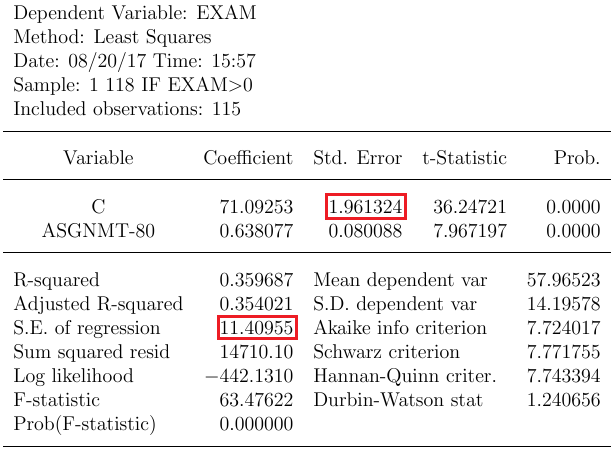
\includegraphics{q1_23}
\end{figure}
\vspace{-\baselineskip}
\noindent therefore,
$$71.0925 \pm 1.9812 \times 11.57$$
$$[48.191,94.009]$$
\noindent We predict with 95\% confidence that a student who scored 80 in their assignment will score between 48.191 and 94.009 in their final exam.

\newpage
\noindent 95\% prediction interval for the exam mark of a student who obtained 80\% \uline{without estimation uncertainty},
$$\hat{exam} \pm t_{0.975,n-k-1} \times se(\hat{e})$$
$$\hat{exam} \pm t_{0.975,n-k-1} \times \sqrt{\hat{\sigma}^2 + \xcancel{(se(\hat{exam}|asgnmt=80))^2}}$$
$$\hat{exam} \pm t_{0.975,n-k-1} \times \sqrt{\hat{\sigma}^2}$$
$$71.0925 \pm 1.9812 \times \sqrt{11.40955^2}$$
$$[48.528,93.672]$$
\noindent With estimation uncertainty, the prediction interval is only slightly larger than without estimation uncertainty.

\newpage
\noindent \textcolor{red}{(d) Specify and estimate a regression model to test whether both the intercept and slope in the regression in part (c) is different for ETC2410 and ETC3440.}

\noindent By including the \uline{dummy variable etc3440}, we have a regression model where the intercept of expected exam score differs between ETC2410 and ETC3440 students holding assignment score constant, $$exam = \beta_0 + \beta_1asgnmt + \delta_0etc3440 + u$$ $$E(exam|asgnmt,etc3440) = \beta_0 + \beta_1asgnmt + \delta_0etc3440$$
\begin{align*}
	E(exam|asgnmt,etc3440=0) &= \beta_0 + \beta_1asgnmt + \delta_0 \times 0 \\
	& = \beta_0 + \beta_1asgnmt
\end{align*}
\begin{align*}
	E(exam|asgnmt,etc3440=1) &= \beta_0 + \beta_1asgnmt + \delta_0 \times 1 \\
	& = (\beta_0 + \delta_0) + \beta_1asgnmt
\end{align*}
\noindent $\delta_0$ is the difference in intercept.

\noindent By including both the \uline{dummy variable and the interaction between $etc3440$ and $asgnmt$}, we have a regression model where both intercept and slope of expected exam score differs between ETC2410 and ETC3440 students holding assignment score constant,
$$exam = \beta_0 + \beta_1asgnmt + \delta_0etc3440 + \delta_1etc3440^*asgnmt + u$$
$$E(exam|asgnmt,etc3440) = \beta_0 + \beta_1asgnmt + \delta_0etc3440 + \delta_1etc3440^*asgnmt $$ \begin{align*}
E(exam|asgnmt,etc3440=0) &= \beta_0 + \beta_1asgnmt + \delta_0 \times 0 + \delta_1\times 0 \\
& = \beta_0 + \beta_1asgnmt
\end{align*}
\begin{align*}
E(exam|asgnmt,etc3440=1) &= \beta_0 + \beta_1asgnmt + \delta_0 \times 1 + \delta_1asgnmt \\
& = (\beta_0 + \delta_0) + (\beta_1 + \delta_1)asgnmt
\end{align*}
\noindent $\delta_0$ and $\delta_1$ represent the different in intercept and slope respectively.

\newpage
\noindent \textcolor{red}
{
	Testing whether the intercept and/or slope is different between ETC3440 and ETC2410 students.
}

\noindent If there is no difference between intercepts and slopes for the expectation of exam mark between ETC3440 and ETC2410 students (holding assignment mark constant),
$$\delta_0 = \delta_1 = 0$$
\noindent and if the intercept and/or slope is different,
$$\delta_0 \neq 0\ and/or\ \delta_1 \neq 0$$
\noindent Since this is a test of 2 linear restrictions and the alternative is a two-sided, we use the F-test. When performing an F-test, we need to estimate the unrestricted and restricted model to obtain $SSR_{ur}$ and $SSR_r$.

\noindent \noindent \textbf{Unrestricted model (the model before imposing restrictions)}:
$$exam = \beta_0 + \beta_1asgnmt + \delta_0etc3440 + \delta_1etc3440^*asgnmt + u$$

\noindent \textbf{Restricted model (the model after imposing restrictions)}:
\begin{align*}
	exam &= \beta_0 + \beta_1asgnmt + 0\times etc3440 + 0\times etc3440^*asgnmt + u \\
	&= \beta_0 + \beta_1asgnmt + u
\end{align*}

\noindent To estimate the unrestricted model from the Command window,
$$ls\ exam\ c\ asgnmt\ etc3440\ etc3440^*asgnmt$$
\begin{figure}[H]
	\centering
	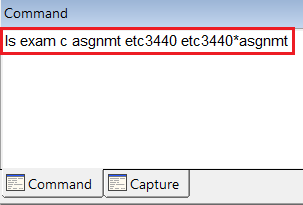
\includegraphics{q1_24}
\end{figure}
\vspace{-\baselineskip}
%%%%%%%%%% TABLE OBJECT %%%%%%%%%%
\begin{table}[H]
	\centering
	\begin{tabular}{lrrrr}
		\multicolumn{3}{l}{Dependent Variable: EXAM}&\multicolumn{1}{c}{}&\multicolumn{1}{c}{}\\
		\multicolumn{3}{l}{Method: Least Squares}&\multicolumn{1}{c}{}&\multicolumn{1}{c}{}\\
		\multicolumn{3}{l}{Sample: 1 118 IF EXAM\textgreater 0}&\multicolumn{1}{c}{}&\multicolumn{1}{c}{}\\
		\multicolumn{3}{l}{Included observations: 115}&\multicolumn{1}{c}{}&\multicolumn{1}{c}{}\\
		[4.5pt] \hline \\ [-4.5pt]
		\multicolumn{1}{c}{Variable}&\multicolumn{1}{r}{Coefficient}&\multicolumn{1}{r}{Std. Error}&\multicolumn{1}{r}{t-Statistic}&\multicolumn{1}{r}{Prob.}\\
		[4.5pt] \hline \\ [-4.5pt]
		\multicolumn{1}{c}{C}&\multicolumn{1}{r}{$13.72129$}&\multicolumn{1}{r}{$5.657110$}&\multicolumn{1}{r}{$2.425495$}&\multicolumn{1}{r}{$0.0169$}\\
		\multicolumn{1}{c}{ASGNMT}&\multicolumn{1}{r}{$0.768005$}&\multicolumn{1}{r}{$0.093077$}&\multicolumn{1}{r}{$8.251292$}&\multicolumn{1}{r}{$0.0000$}\\
		\multicolumn{1}{c}{ETC3440}&\multicolumn{1}{r}{$21.87665$}&\multicolumn{1}{r}{$10.38634$}&\multicolumn{1}{r}{$2.106291$}&\multicolumn{1}{r}{$0.0374$}\\
		\multicolumn{1}{c}{ETC3440*ASGNMT}&\multicolumn{1}{r}{$-0.420274$}&\multicolumn{1}{r}{$0.170347$}&\multicolumn{1}{r}{$-2.467161$}&\multicolumn{1}{r}{$0.0151$}\\
		[4.5pt] \hline \\ [-4.5pt]
		\multicolumn{1}{l}{R-squared}&\multicolumn{1}{r}{$0.404915$}&\multicolumn{2}{l}{Mean dependent var}&\multicolumn{1}{r}{$57.96523$}\\
		\multicolumn{1}{l}{Adjusted R-squared}&\multicolumn{1}{r}{$0.388831$}&\multicolumn{2}{l}{S.D. dependent var}&\multicolumn{1}{r}{$14.19578$}\\
		\multicolumn{1}{l}{S.E. of regression}&\multicolumn{1}{r}{$11.09788$}&\multicolumn{2}{l}{Akaike info criterion}&\multicolumn{1}{r}{$7.685548$}\\
		\multicolumn{1}{l}{Sum squared resid}&\multicolumn{1}{r}{$13671.08$}&\multicolumn{2}{l}{Schwarz criterion}&\multicolumn{1}{r}{$7.781024$}\\
		\multicolumn{1}{l}{Log likelihood}&\multicolumn{1}{r}{$-437.9190$}&\multicolumn{2}{l}{Hannan-Quinn criter.}&\multicolumn{1}{r}{$7.724301$}\\
		\multicolumn{1}{l}{F-statistic}&\multicolumn{1}{r}{$25.17594$}&\multicolumn{2}{l}{Durbin-Watson stat}&\multicolumn{1}{r}{$1.282800$}\\
		\multicolumn{1}{l}{Prob(F-statistic)}&\multicolumn{1}{r}{$0.000000$}&\multicolumn{1}{c}{}&\multicolumn{1}{c}{}&\multicolumn{1}{c}{}\\
		[4.5pt] \hline \\ [-4.5pt]
	\end{tabular}
	%\caption{}
	%\label{tab:}
\end{table} \centering $SSR_{ur} = 13671.08$

\justify
%%%%%%%%%% TABLE OBJECT %%%%%%%%%%
\begin{table}[H]
	\centering
	\begin{tabular}{lrrrr}
		\multicolumn{3}{l}{Dependent Variable: EXAM}&\multicolumn{1}{c}{}&\multicolumn{1}{c}{}\\
		\multicolumn{3}{l}{Method: Least Squares}&\multicolumn{1}{c}{}&\multicolumn{1}{c}{}\\
		\multicolumn{3}{l}{Sample: 1 118 IF EXAM\textgreater 0}&\multicolumn{1}{c}{}&\multicolumn{1}{c}{}\\
		\multicolumn{3}{l}{Included observations: 115}&\multicolumn{1}{c}{}&\multicolumn{1}{c}{}\\
		[4.5pt] \hline \\ [-4.5pt]
		\multicolumn{1}{c}{Variable}&\multicolumn{1}{r}{Coefficient}&\multicolumn{1}{r}{Std. Error}&\multicolumn{1}{r}{t-Statistic}&\multicolumn{1}{r}{Prob.}\\
		[4.5pt] \hline \\ [-4.5pt]
		\multicolumn{1}{c}{C}&\multicolumn{1}{r}{$20.04634$}&\multicolumn{1}{r}{$4.876848$}&\multicolumn{1}{r}{$4.110512$}&\multicolumn{1}{r}{$0.0001$}\\
		\multicolumn{1}{c}{ASGNMT}&\multicolumn{1}{r}{$0.638077$}&\multicolumn{1}{r}{$0.080088$}&\multicolumn{1}{r}{$7.967197$}&\multicolumn{1}{r}{$0.0000$}\\
		[4.5pt] \hline \\ [-4.5pt]
		\multicolumn{1}{l}{R-squared}&\multicolumn{1}{r}{$0.359687$}&\multicolumn{2}{l}{Mean dependent var}&\multicolumn{1}{r}{$57.96523$}\\
		\multicolumn{1}{l}{Adjusted R-squared}&\multicolumn{1}{r}{$0.354021$}&\multicolumn{2}{l}{S.D. dependent var}&\multicolumn{1}{r}{$14.19578$}\\
		\multicolumn{1}{l}{S.E. of regression}&\multicolumn{1}{r}{$11.40955$}&\multicolumn{2}{l}{Akaike info criterion}&\multicolumn{1}{r}{$7.724017$}\\
		\multicolumn{1}{l}{Sum squared resid}&\multicolumn{1}{r}{$14710.10$}&\multicolumn{2}{l}{Schwarz criterion}&\multicolumn{1}{r}{$7.771755$}\\
		\multicolumn{1}{l}{Log likelihood}&\multicolumn{1}{r}{$-442.1310$}&\multicolumn{2}{l}{Hannan-Quinn criter.}&\multicolumn{1}{r}{$7.743394$}\\
		\multicolumn{1}{l}{F-statistic}&\multicolumn{1}{r}{$63.47622$}&\multicolumn{2}{l}{Durbin-Watson stat}&\multicolumn{1}{r}{$1.240656$}\\
		\multicolumn{1}{l}{Prob(F-statistic)}&\multicolumn{1}{r}{$0.000000$}&\multicolumn{1}{c}{}&\multicolumn{1}{c}{}&\multicolumn{1}{c}{}\\
		[4.5pt] \hline \\ [-4.5pt]
	\end{tabular}
	%\caption{Regression output of the \textbf{restricted model}.}
	%\label{tab:}
\end{table}\centering $SSR_{r} = 14710.10$

\justify
\noindent \textbf{State the null and alternative hypothesis}
\begin{align*}
	&H_0: \delta_0 = \delta_1 = 0 \\
	&H_1: \delta_0 \neq 0\ and/or\ \delta_1 \neq 0
\end{align*}

\noindent \textbf{The test statistic and its distribution under $H_0$}
$$F = \dfrac{(SSR_r - SSR_{ur})/q}{SSR_{ur}/(n-k-1)} = \dfrac{(SSR_r - SSR_{ur})/2}{SSR_{ur}/(115-3-1)} \sim F_{2,111} \quad under\ H_0$$
\begin{align*}
n &= sample\ size = 115 \\
k &= number\ of\ regressors\ in\ the\ unrestricted\ model = 4 \\
q &= number\ of\ restrictions\ = 2 \\
SSR_{r} &= sum\ of\ squared\ residuals\ from\ estimated\ restricted\ model \\
SSR_{ur} &= sum\ of\ squared\ residuals\ from\ estimated\ unrestricted\ model
\end{align*}

\noindent \textbf{Calculate the test statistic}
$$F_{calc} = \dfrac{(SSR_r - SSR_{ur})/2}{SSR_{ur}/(111)} = \dfrac{(14710.10-13671.08)/2}{13671.08/(111)} = 4.2181 $$


\noindent \textbf{Critical value and rejection region}

\noindent $5\%\ significance\ level\ \to \alpha = 0.05$

\noindent To obtain the critical value using the Stats Table, locate the F distribution table at the 5\% significance level,
$$Numerator\ d.o.f = 2$$
$$Denominator\ d.o.f = 111$$
\noindent Since 111 is not in the table, we take a conservative approach and choose the closest available degrees of freedom less than 111 i.e. $d.o.f=90$. 
\begin{figure}[H]
	\centerline{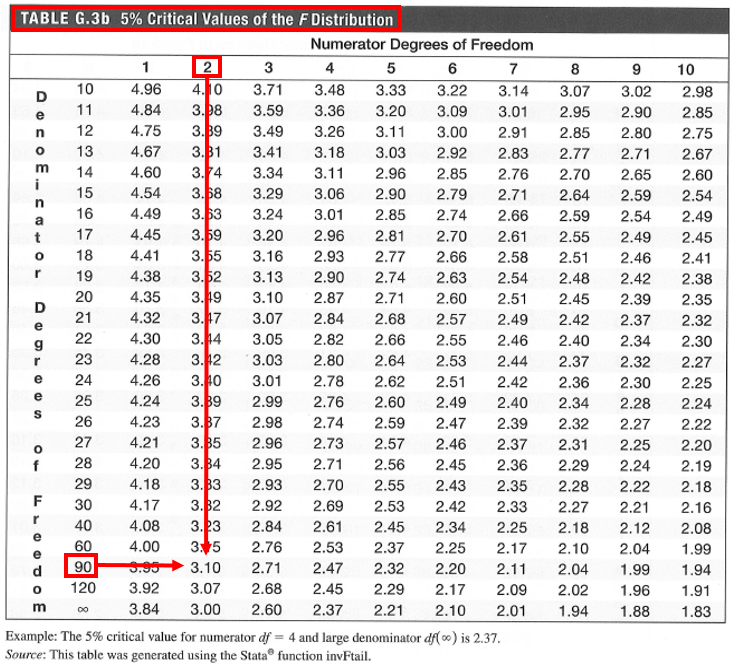
\includegraphics{q1_25}}
\end{figure}
\vspace{-\baselineskip}
\noindent To obtain the critical value using EViews,
$$Command\ window:\ scalar\ cvf1=@qfdist(0.95,2,111)$$
\begin{figure}[H]
	\centering
	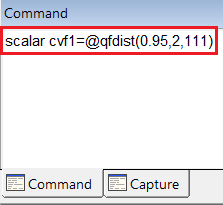
\includegraphics{q1_26}
\end{figure}
\vspace{-\baselineskip}
\begin{figure}[H]
	\centering
	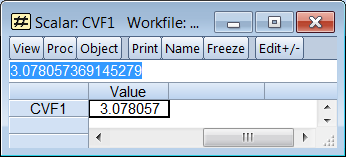
\includegraphics{q1_27}
\end{figure}
\vspace{-\baselineskip}
$$F_{crit}\ (from\ Stat\ Table) = 3.10$$
$$F_{crit}\ (from\ EViews) = 3.0781$$

\noindent Rejection rule: 

\noindent Comparing the calculated test statistic with the critical value, we reject $H_0$ if,
$$F_{calc} > F_{crit}$$

\noindent \textbf{Conclusion}

\noindent Since $F_{calc}=4.2181 > F_{crit}=3.0781$, we reject the null at the 5\% significance level and conclude that there is sufficient evidence from our sample to suggest that the expectation of exam mark differs for ETC3440 and ETC2410 students either in the intercept and/or the slope, holding assignment mark constant.

\newpage
\noindent \textcolor{red}
{
	From the unrestricted regression results, obtain the estimate of the intercept and slope for ETC2410 and for ETC3440 regression lines.
}
%%%%%%%%%% TABLE OBJECT %%%%%%%%%%
\begin{table}[H]
	\centering
	\begin{tabular}{lrrrr}
		\multicolumn{3}{l}{Dependent Variable: EXAM}&\multicolumn{1}{c}{}&\multicolumn{1}{c}{}\\
		\multicolumn{3}{l}{Method: Least Squares}&\multicolumn{1}{c}{}&\multicolumn{1}{c}{}\\
		\multicolumn{3}{l}{Sample: 1 118 IF EXAM\textgreater 0}&\multicolumn{1}{c}{}&\multicolumn{1}{c}{}\\
		\multicolumn{3}{l}{Included observations: 115}&\multicolumn{1}{c}{}&\multicolumn{1}{c}{}\\
		[4.5pt] \hline \\ [-4.5pt]
		\multicolumn{1}{c}{Variable}&\multicolumn{1}{r}{Coefficient}&\multicolumn{1}{r}{Std. Error}&\multicolumn{1}{r}{t-Statistic}&\multicolumn{1}{r}{Prob.}\\
		[4.5pt] \hline \\ [-4.5pt]
		\multicolumn{1}{c}{C}&\multicolumn{1}{r}{$13.72129$}&\multicolumn{1}{r}{$5.657110$}&\multicolumn{1}{r}{$2.425495$}&\multicolumn{1}{r}{$0.0169$}\\
		\multicolumn{1}{c}{ASGNMT}&\multicolumn{1}{r}{$0.768005$}&\multicolumn{1}{r}{$0.093077$}&\multicolumn{1}{r}{$8.251292$}&\multicolumn{1}{r}{$0.0000$}\\
		\multicolumn{1}{c}{ETC3440}&\multicolumn{1}{r}{$21.87665$}&\multicolumn{1}{r}{$10.38634$}&\multicolumn{1}{r}{$2.106291$}&\multicolumn{1}{r}{$0.0374$}\\
		\multicolumn{1}{c}{ETC3440*ASGNMT}&\multicolumn{1}{r}{$-0.420274$}&\multicolumn{1}{r}{$0.170347$}&\multicolumn{1}{r}{$-2.467161$}&\multicolumn{1}{r}{$0.0151$}\\
		[4.5pt] \hline \\ [-4.5pt]
		\multicolumn{1}{l}{R-squared}&\multicolumn{1}{r}{$0.404915$}&\multicolumn{2}{l}{Mean dependent var}&\multicolumn{1}{r}{$57.96523$}\\
		\multicolumn{1}{l}{Adjusted R-squared}&\multicolumn{1}{r}{$0.388831$}&\multicolumn{2}{l}{S.D. dependent var}&\multicolumn{1}{r}{$14.19578$}\\
		\multicolumn{1}{l}{S.E. of regression}&\multicolumn{1}{r}{$11.09788$}&\multicolumn{2}{l}{Akaike info criterion}&\multicolumn{1}{r}{$7.685548$}\\
		\multicolumn{1}{l}{Sum squared resid}&\multicolumn{1}{r}{$13671.08$}&\multicolumn{2}{l}{Schwarz criterion}&\multicolumn{1}{r}{$7.781024$}\\
		\multicolumn{1}{l}{Log likelihood}&\multicolumn{1}{r}{$-437.9190$}&\multicolumn{2}{l}{Hannan-Quinn criter.}&\multicolumn{1}{r}{$7.724301$}\\
		\multicolumn{1}{l}{F-statistic}&\multicolumn{1}{r}{$25.17594$}&\multicolumn{2}{l}{Durbin-Watson stat}&\multicolumn{1}{r}{$1.282800$}\\
		\multicolumn{1}{l}{Prob(F-statistic)}&\multicolumn{1}{r}{$0.000000$}&\multicolumn{1}{c}{}&\multicolumn{1}{c}{}&\multicolumn{1}{c}{}\\
		[4.5pt] \hline \\ [-4.5pt]
	\end{tabular}
	%\caption{Regression output of the \textbf{unrestricted model}.}
	%\label{tab:}
\end{table}

\vspace{-\baselineskip}
\noindent Regression line of final exam mark against assignment mark for ETC2410 students:
\begin{align*}
	\widehat{E(exam|asgnmt,etc3440=0)} &= \hat{\beta}_0 + \hat{\beta}_1asgnmt \\
	&= 13.7213 + 0.7680asgnmt 
\end{align*}


\noindent Regression line of final exam mark against assignment mark for ETC3440 students:
\begin{align*}
\widehat{E(exam|asgnmt,etc3440=1)} &= (\hat{\beta}_0 + \hat{\delta}_0) + (\hat{\beta}_1 + \hat{\delta}_1)asgnmt \\
&= (13.7213+21.8767) + (0.7680-0.4203)asgnmt \\
&= 35.5979+0.3477asgnmt
\end{align*}

\newpage
\noindent \textcolor{red}{(e) Estimate two separate models to predict exam mark based on assignment mark, one for ETC2410 students and another for ETC3440 students.}
$$exam = \beta_0 + \beta_1asgnmt + u$$
\noindent To estimate the model  based on sample of ETC3440 students only:
$$Quick \to Estimate\ Equation$$
$$Equation\ estimation: exam\ c\ asgnmt$$
$$Sample: 1\ 118\ if\ exam>0\ and\ etc3440=1$$
\begin{figure}[H]
	\centering
	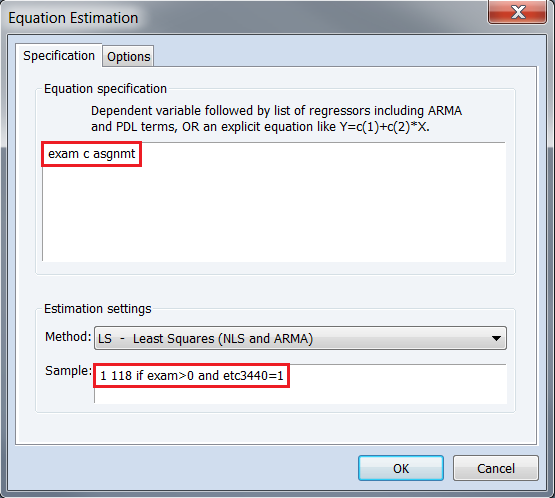
\includegraphics{q1_28}
\end{figure}
\vspace{-\baselineskip}
%%%%%%%%%% TABLE OBJECT %%%%%%%%%%
\begin{table}[H]
	\centering
	\begin{tabular}{lrrrr}
		\multicolumn{3}{l}{Dependent Variable: EXAM}&\multicolumn{1}{c}{}&\multicolumn{1}{c}{}\\
		\multicolumn{3}{l}{Method: Least Squares}&\multicolumn{1}{c}{}&\multicolumn{1}{c}{}\\
		\multicolumn{4}{l}{Sample: 1 118 IF EXAM\textgreater 0 AND ETC3440=1}&\multicolumn{1}{c}{}\\
		\multicolumn{3}{l}{Included observations: 48}&\multicolumn{1}{c}{}&\multicolumn{1}{c}{}\\
		[4.5pt] \hline \\ [-4.5pt]
		\multicolumn{1}{c}{Variable}&\multicolumn{1}{r}{Coefficient}&\multicolumn{1}{r}{Std. Error}&\multicolumn{1}{r}{t-Statistic}&\multicolumn{1}{r}{Prob.}\\
		[4.5pt] \hline \\ [-4.5pt]
		\multicolumn{1}{c}{C}&\multicolumn{1}{r}{$35.59794$}&\multicolumn{1}{r}{$8.108920$}&\multicolumn{1}{r}{$4.389973$}&\multicolumn{1}{r}{$0.0001$}\\
		\multicolumn{1}{c}{ASGNMT}&\multicolumn{1}{r}{$0.347731$}&\multicolumn{1}{r}{$0.132817$}&\multicolumn{1}{r}{$2.618119$}&\multicolumn{1}{r}{$0.0119$}\\
		[4.5pt] \hline \\ [-4.5pt]
		\multicolumn{1}{l}{R-squared}&\multicolumn{1}{r}{$0.129687$}&\multicolumn{2}{l}{Mean dependent var}&\multicolumn{1}{r}{$56.46599$}\\
		\multicolumn{1}{l}{Adjusted R-squared}&\multicolumn{1}{r}{$0.110767$}&\multicolumn{2}{l}{S.D. dependent var}&\multicolumn{1}{r}{$10.95598$}\\
		\multicolumn{1}{l}{S.E. of regression}&\multicolumn{1}{r}{$10.33139$}&\multicolumn{2}{l}{Akaike info criterion}&\multicolumn{1}{r}{$7.549025$}\\
		\multicolumn{1}{l}{Sum squared resid}&\multicolumn{1}{r}{$4909.934$}&\multicolumn{2}{l}{Schwarz criterion}&\multicolumn{1}{r}{$7.626992$}\\
		\multicolumn{1}{l}{Log likelihood}&\multicolumn{1}{r}{$-179.1766$}&\multicolumn{2}{l}{Hannan-Quinn criter.}&\multicolumn{1}{r}{$7.578489$}\\
		\multicolumn{1}{l}{F-statistic}&\multicolumn{1}{r}{$6.854548$}&\multicolumn{2}{l}{Durbin-Watson stat}&\multicolumn{1}{r}{$0.971504$}\\
		\multicolumn{1}{l}{Prob(F-statistic)}&\multicolumn{1}{r}{$0.011930$}&\multicolumn{1}{c}{}&\multicolumn{1}{c}{}&\multicolumn{1}{c}{}\\
		[4.5pt] \hline \\ [-4.5pt]
	\end{tabular}
	%\caption{Regression output of $exam$ on a constant and $asgnmt$ from the sample of ETC3440 students only.}
	%\label{tab:}
\end{table}

\vspace{-\baselineskip}
$$\widehat{exam} = \underset{(8.1089)}{35.5979} + \underset{(0.1328)}{0.3477}asgnmt$$
$$SSR_{with\ etc3440\ students\ only} = 4909.934$$

\noindent To estimate the model  based on sample of ETC2410 students only:
$$Quick \to Estimate\ Equation$$
$$Equation\ estimation: exam\ c\ asgnmt$$
$$Sample: 1\ 118\ if\ exam>0\ and\ etc3440=1$$

\begin{figure}[H]
	\centering
	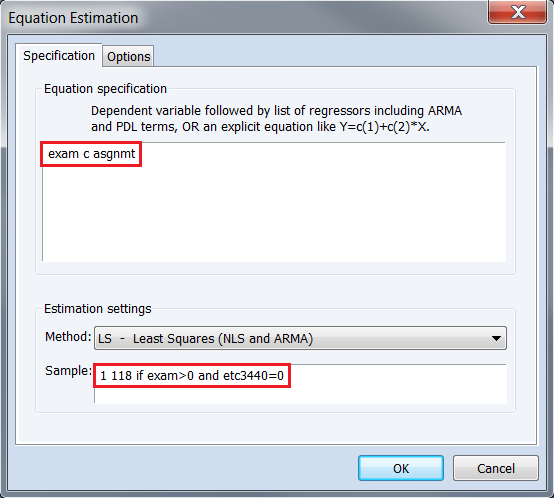
\includegraphics{q1_29}
\end{figure}
\vspace{-\baselineskip}
%%%%%%%%%% TABLE OBJECT %%%%%%%%%%
\begin{table}[H]
	\centering
	\begin{tabular}{lrrrr}
		\multicolumn{3}{l}{Dependent Variable: EXAM}&\multicolumn{1}{c}{}&\multicolumn{1}{c}{}\\
		\multicolumn{3}{l}{Method: Least Squares}&\multicolumn{1}{c}{}&\multicolumn{1}{c}{}\\
		\multicolumn{4}{l}{Sample: 1 118 IF EXAM\textgreater 0 AND ETC3440=0}&\multicolumn{1}{c}{}\\
		\multicolumn{3}{l}{Included observations: 67}&\multicolumn{1}{c}{}&\multicolumn{1}{c}{}\\
		[4.5pt] \hline \\ [-4.5pt]
		\multicolumn{1}{c}{Variable}&\multicolumn{1}{r}{Coefficient}&\multicolumn{1}{r}{Std. Error}&\multicolumn{1}{r}{t-Statistic}&\multicolumn{1}{r}{Prob.}\\
		[4.5pt] \hline \\ [-4.5pt]
		\multicolumn{1}{c}{C}&\multicolumn{1}{r}{$13.72129$}&\multicolumn{1}{r}{$5.918047$}&\multicolumn{1}{r}{$2.318550$}&\multicolumn{1}{r}{$0.0236$}\\
		\multicolumn{1}{c}{ASGNMT}&\multicolumn{1}{r}{$0.768005$}&\multicolumn{1}{r}{$0.097370$}&\multicolumn{1}{r}{$7.887477$}&\multicolumn{1}{r}{$0.0000$}\\
		[4.5pt] \hline \\ [-4.5pt]
		\multicolumn{1}{l}{R-squared}&\multicolumn{1}{r}{$0.489043$}&\multicolumn{2}{l}{Mean dependent var}&\multicolumn{1}{r}{$59.03932$}\\
		\multicolumn{1}{l}{Adjusted R-squared}&\multicolumn{1}{r}{$0.481182$}&\multicolumn{2}{l}{S.D. dependent var}&\multicolumn{1}{r}{$16.11819$}\\
		\multicolumn{1}{l}{S.E. of regression}&\multicolumn{1}{r}{$11.60977$}&\multicolumn{2}{l}{Akaike info criterion}&\multicolumn{1}{r}{$7.770968$}\\
		\multicolumn{1}{l}{Sum squared resid}&\multicolumn{1}{r}{$8761.143$}&\multicolumn{2}{l}{Schwarz criterion}&\multicolumn{1}{r}{$7.836779$}\\
		\multicolumn{1}{l}{Log likelihood}&\multicolumn{1}{r}{$-258.3274$}&\multicolumn{2}{l}{Hannan-Quinn criter.}&\multicolumn{1}{r}{$7.797009$}\\
		\multicolumn{1}{l}{F-statistic}&\multicolumn{1}{r}{$62.21230$}&\multicolumn{2}{l}{Durbin-Watson stat}&\multicolumn{1}{r}{$1.442208$}\\
		\multicolumn{1}{l}{Prob(F-statistic)}&\multicolumn{1}{r}{$0.000000$}&\multicolumn{1}{c}{}&\multicolumn{1}{c}{}&\multicolumn{1}{c}{}\\
		[4.5pt] \hline \\ [-4.5pt]
	\end{tabular}
	%\caption{Regression output on $exam$ on a constant and $asgnmt$ from the sample of ETC2410 students only.}
	%\label{tab:}
\end{table}

\vspace{-\baselineskip}
$$\widehat{exam} = \underset{(5.9180)}{13.7213} + \underset{(0.0974)}{0.7680}asgnmt$$
$$SSR_{with\ etc2410\ students\ only} = 8761.143$$

\noindent \textcolor{red}
{
	Compare the estimates of the intercept and slope you obtain here with what you obtained in part (d) and discuss.
}

\noindent From part (d), we regressed $exam$ on a constant, $asgnmt$, $etc3440$ and $etc3440^*asgnmt$ using the sample with both ETC3440 and ETC2410 students,
$$\widehat{exam} = \underset{(5.6571)}{13.7213} + \underset{(0.0931)}{0.7680}asgnmt + \underset{(10.3863)}{21.8767}etc3440 - \underset{(0.1703)}{0.4204}etc3440^*asgnmt$$
$$SSR_{ur} = 13671.08$$
\noindent ETC2410 students only,
$$\widehat{exam} = \underset{(5.9180)}{13.7213} + \underset{(0.0974)}{0.7680}asgnmt$$
\noindent ETC3440 students only,
$$\widehat{exam} = \underset{(8.1089)}{35.5979} + \underset{(0.1328)}{0.3477}asgnmt$$

\noindent What we find when comparing each model,
$$\hat{\beta}_{0\ with\ etc2410\ students\ only} = \hat{\beta}_{0\ part(d)}$$
$$\hat{\beta}_{1\ with\ etc2410\ students\ only} = \hat{\beta}_{1\ part(d)}$$
$$\hat{\beta}_{0\ with\ etc3440\ students\ only} = \hat{\beta}_{0\ part(d)} + \hat{\delta}_{0\ part(d)}$$
$$\hat{\beta}_{1\ with\ etc3440\ students\ only} = \hat{\beta}_{1\ part(d)} + \hat{\delta}_{1\ part(d)}$$
\noindent The intuitive reason for why we observe this relationship: 
\begin{itemize}
	\item The parameters for the ETC2410 group (the parameters you see when the dummy variable equals to 0) only affects the $SSR$ of the ETC2410 group.
	\item Similarly, the parameters for the ETC3440 group (the parameters you see when the dummy variable equals to 1) only affects the $SSR$ of the ETC3440 group.
	\item There is no common parameter that enters both i.e. each group's parameters are separate.
\end{itemize}
\noindent As such, the OLS estimator achieves the smallest $SSR$ for the model of both groups, when the $SSR$ of the model of each individual group is minimised.
$$SSR_{with\ etc2410\ students\ only} + SSR_{with\ etc3440\ students\ only} = SSR_{ur}$$
$$8761.143 + 4909.934 = 13671.08$$

\newpage
\noindent \textcolor{red}{(f) Consider the estimated intercept and slope of ETC2410 students in part (d) and part (e). While the numerical values are the same, their standard errors are not. Discuss why they are different, and which one you would prefer to use to construct a 95\% confidence interval for the slope parameter for ETC2410 students.}

\noindent The standard error of $\boldsymbol{\hat{\beta}}$,
$$\widehat{var({\boldsymbol{\hat{\beta}}|\boldsymbol{X}})} = \hat{\sigma}^2(\boldsymbol{X'X})^{-1} \quad (estimated\ variance-covariance\ matrix\ of\ \boldsymbol{\hat{\beta}})$$
$$se(\boldsymbol{\hat{\beta}}) = \sqrt{\hat{\sigma}^2(\boldsymbol{X'X})^{-1}}$$
\noindent depends on,
$$\hat{\sigma}^2 = \dfrac{\sum_{i}^{n}\hat{u}_{i}^{2}}{n-k-1} = \dfrac{SSR}{n-k-1} = unbiased\ estimator\ of\ var(\boldsymbol{u}|\boldsymbol{X})$$
and since $\hat{\sigma}^2$ differs between each model,
$$\hat{\sigma}^2_{with\ etc2410\ students\ only} = 11.6098^2 \neq \hat{\sigma}^2_{ur} = 11.0997^2$$
\noindent We need to consider which standard error to use when constructing the 95\% confidence interval of the slope parameter for ETC2410 students,
$$\hat{\beta}_1 \pm t_{0.975} \times se(\hat{\beta}_1)_{with\ etc2410\ students\ only}$$
$$OR$$
$$\hat{\beta}_1 \pm t_{0.975} \times se(\hat{\beta}_1)_{unrestricted\ with\ both\ etc2410\ and\ etc3440\ sample}$$
\noindent From question (d), we found that there was sufficient evidence to suggest that the conditional expectation of exam mark, after controlling for assignment, mark differs between ETC2410 and ETC3440 students, $$E(exam|asgnmt, etc3440=1) \neq E(exam|asgnmt, etc3440=0) $$ so there is no compelling reason to insist that $var(\boldsymbol{u}|\boldsymbol{X})$ (which is equal to $var(\boldsymbol{y}|\textbf{\textit{X}})$) should be the same across both groups $\therefore$ we should base our confidence interval of the slope parameter of ETC2410 students using $se(\hat{\beta}_1)_{with\ etc2410\ students\ only}$ and not $se(\hat{\beta}_1)_{unrestricted\ with\ both\ etc2410\ and\ etc3440\ sample}$.



\end{document}
